\documentclass{standalone}
\usepackage[utf8]{inputenc}
\usepackage{tikz}
\usetikzlibrary{shapes.geometric, arrows}
\begin{document}

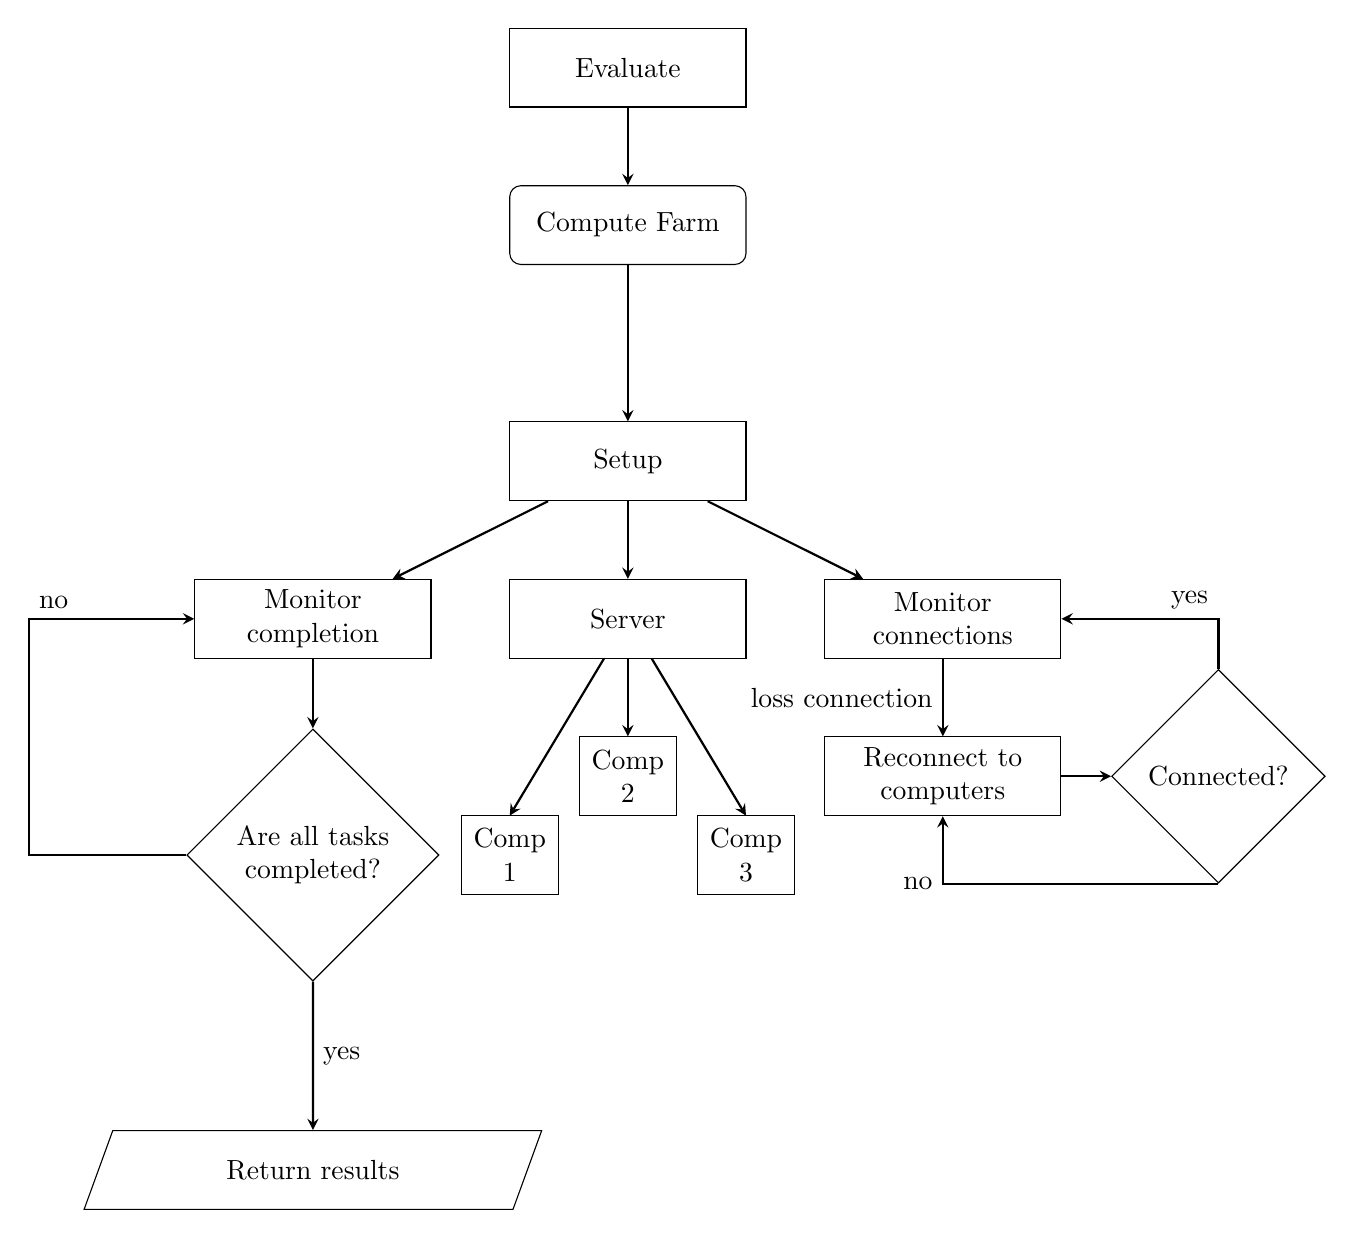
\begin{tikzpicture}[node distance=2cm]

\tikzstyle{program} = [rectangle, rounded corners, minimum width=3cm, minimum height=1cm,text centered, draw=black]
\tikzstyle{io} = [trapezium, trapezium left angle=70, trapezium right angle=110, minimum width=3cm, minimum height=1cm, text centered, draw=black]
\tikzstyle{process} = [rectangle, minimum width=3cm, minimum height=1cm, text centered, text width=2.5cm, draw=black]
\tikzstyle{comp} = [rectangle, minimum width=1cm, minimum height=1cm, text centered, text width=1cm, draw=black]
\tikzstyle{decision} = [diamond, minimum width=2.5cm, minimum height=0.5cm,text width =2cm, text centered, draw=black]
\tikzstyle{arrow} = [thick,->,>=stealth]

\node (evaluate) [process] {Evaluate};
\node (compute)  [program, below of = evaluate]             {Compute Farm};
\node (setup)    [process, below of = compute, yshift=-1cm] {Setup};
\node (server)   [process, below of = setup]                {Server};
\node (Monitor)  [process, below of = setup, xshift=-4cm]   {Monitor completion};
\node (Monitor2) [process, below of = setup, xshift=4cm]    {Monitor connections};
\node (connect)  [process, below of = Monitor2]             {Reconnect to computers};

\node (dec1)     [decision, below of = Monitor, yshift = -1cm]  {Are all tasks completed?};
\node (dec2)     [decision, right of = connect,xshift =1.5cm] {Connected?};

\node (comp1) [comp, below of=server,yshift=-1cm,xshift=-1.5cm]  {Comp 1};
\node (comp2) [comp, below of=server]                          {Comp 2};
\node (comp3) [comp, below of=server,yshift=-1cm,xshift=1.5cm]   {Comp 3};

\node (return) [io, below of =dec1,yshift=-2cm] {Return results};

\draw [arrow] (evaluate) -- (compute);
\draw [arrow] (compute) -- (setup);
\draw [arrow] (setup) -- (server);
\draw [arrow] (setup) -- (Monitor);
\draw [arrow] (setup) -- (Monitor2);

\draw [arrow] (Monitor) -- (dec1);
\draw [arrow] (dec1.south) --node[anchor=west] {yes} (return);
\draw [arrow] (dec1.west)  --+(-2,0)|- node[anchor=south west] {no} (Monitor.west);


\draw [arrow] (Monitor2) -- node[anchor=east] {loss connection} (connect);
\draw [arrow] (connect) -- (dec2);
\draw [arrow] (dec2.south) -| node[anchor=east] {no} (connect.south);
\draw [arrow] (dec2.north) |- node[anchor=south east] {yes} (Monitor2.east);

\draw [arrow] (server) --+(-1.5,-2.5) (comp1);
\draw [arrow] (server) -- (comp2);
\draw [arrow] (server) --+(1.5,-2.5) (comp3);


\end{tikzpicture}

\end{document}

